\documentclass[12pt]{article}
\usepackage{graphicx}
\usepackage{hyperref}
\usepackage{eso-pic} 
\usepackage{lipsum} 
\usepackage{listings}
\usepackage[linesnumbered,ruled]{algorithm2e}

\setlength{\parindent}{0em}
\setlength{\parskip}{1em}
\definecolor{pblue}{rgb}{0.13,0.13,1}
\definecolor{pgreen}{rgb}{0,0.5,0}
\definecolor{pred}{rgb}{0.9,0,0}
\definecolor{backcolour}{rgb}{0.95,0.95,0.92}
\lstset{language=Java,
	backgroundcolor=\color{backcolour},
	commentstyle=\color{pgreen},
	keywordstyle=\color{pblue},
	stringstyle=\color{pred},
	basicstyle=\ttfamily,
	numbers=left,
	numberstyle=\tiny,
	frame=single,
	title=\lstname
}

\title{Rapport Projet \\Complément POO \\ \textbf{PUZZLE} }
\author{ ATTY Abla Cathérine Gloria\\ Erwan Phillipe MENSAH \\ TOURE Papa Samba Khary \\Daouda TRAORE}
\renewcommand*\contentsname{Table des matières}
\date{}
\begin{document}
\AddToShipoutPicture*
{\put(440,650){
\includegraphics[width=6cm,height=6cm]{logo.jpg}}}
\maketitle
\mbox{}
\vfill
L2 Informatique 2021-2022 Université Caen Basse-Normandie.

\newpage
\tableofcontents

\newpage
\section{Introduction}

Ce rapport a pour objectif de décrire le processus de conception d'une application de jeux
dotée d'une interface graphique qui consiste en un puzzle à glissière(voir image ci dessous).

Le jeux consiste à faire glisser les cases adjacentes à la case vide qui en fonction de la situation 
peut varier entre \textbf{deux} à \textbf{quatre} possibilités. Le jeux se termine une fois 
l'image est reconstituée ou une fois que l'on a retrouvé le bon ordre des cases.

Le but du devoir est donc la conception d'une telle application mais intrégralement realisée
en utilisant l'architecture \textbf{\textit{Model-View-Controller}} (\textbf{MVC}) dont nous 
reparlerons plus en detail plus tard.   

Ce rapport contient l'ensemble des éléments ayant permis la conception du modèle, de la 
vue et du contrôleur, du mode fonctionnement le l'architecture \textbf{MVC}, ainsi 
que comment le travail fut répartit entre les quatre membres du groupe.
\begin{figure}[h!]
	\begin{center}
		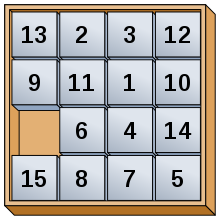
\includegraphics[width=0.5\textwidth]{taquin.png}
	\end{center}
	\caption{Exemple Taquin}
	\label{taquin}
\end{figure}

\section{Répartition du travail}

ATTY : 
\begin{itemize}
	\item View
	\item Controller
	\item Rapport
\end{itemize}
Erwan MENSAH :
\begin{itemize}
	\item Model
	\item Controller
	\item Rapport
\end{itemize}
Daouda TRAORE :
\begin{itemize}
	\item View
	\item Controller
	\item Rapport
\end{itemize}
TOURE Papa :
\begin{itemize}
	\item Model
	\item View
	\item Controller
	\item Rapport
\end{itemize}
Plutôt qu'une répartition en groupe c'était plutôt un travail collectif dans tous l'ensemble du projet.

\section{Architecture du projet}
\subsection{Description du pattern MVC}
L'architecture \textbf{MVC} (\textit{Model-View-Controller}) spécifie q'une application consiste en un
\textbf{\textit{Modèle}} contenant les données et les différentes fonctions de l'application, d'une
\textbf{\textit{Vue}} assurant la présentation de l'information et d'un \textbf{\textit{Contrôleur}}
gérant l'information.

La principale motivation dérrière une telle architecture etait de permettre la création d'un interface
graphique pour n'importe quel type d'objet. De nos jours le pattern MVC est adopté dans la majorité des applications
et des langages de programmation.
\begin{figure}[h!]
	\begin{center}
		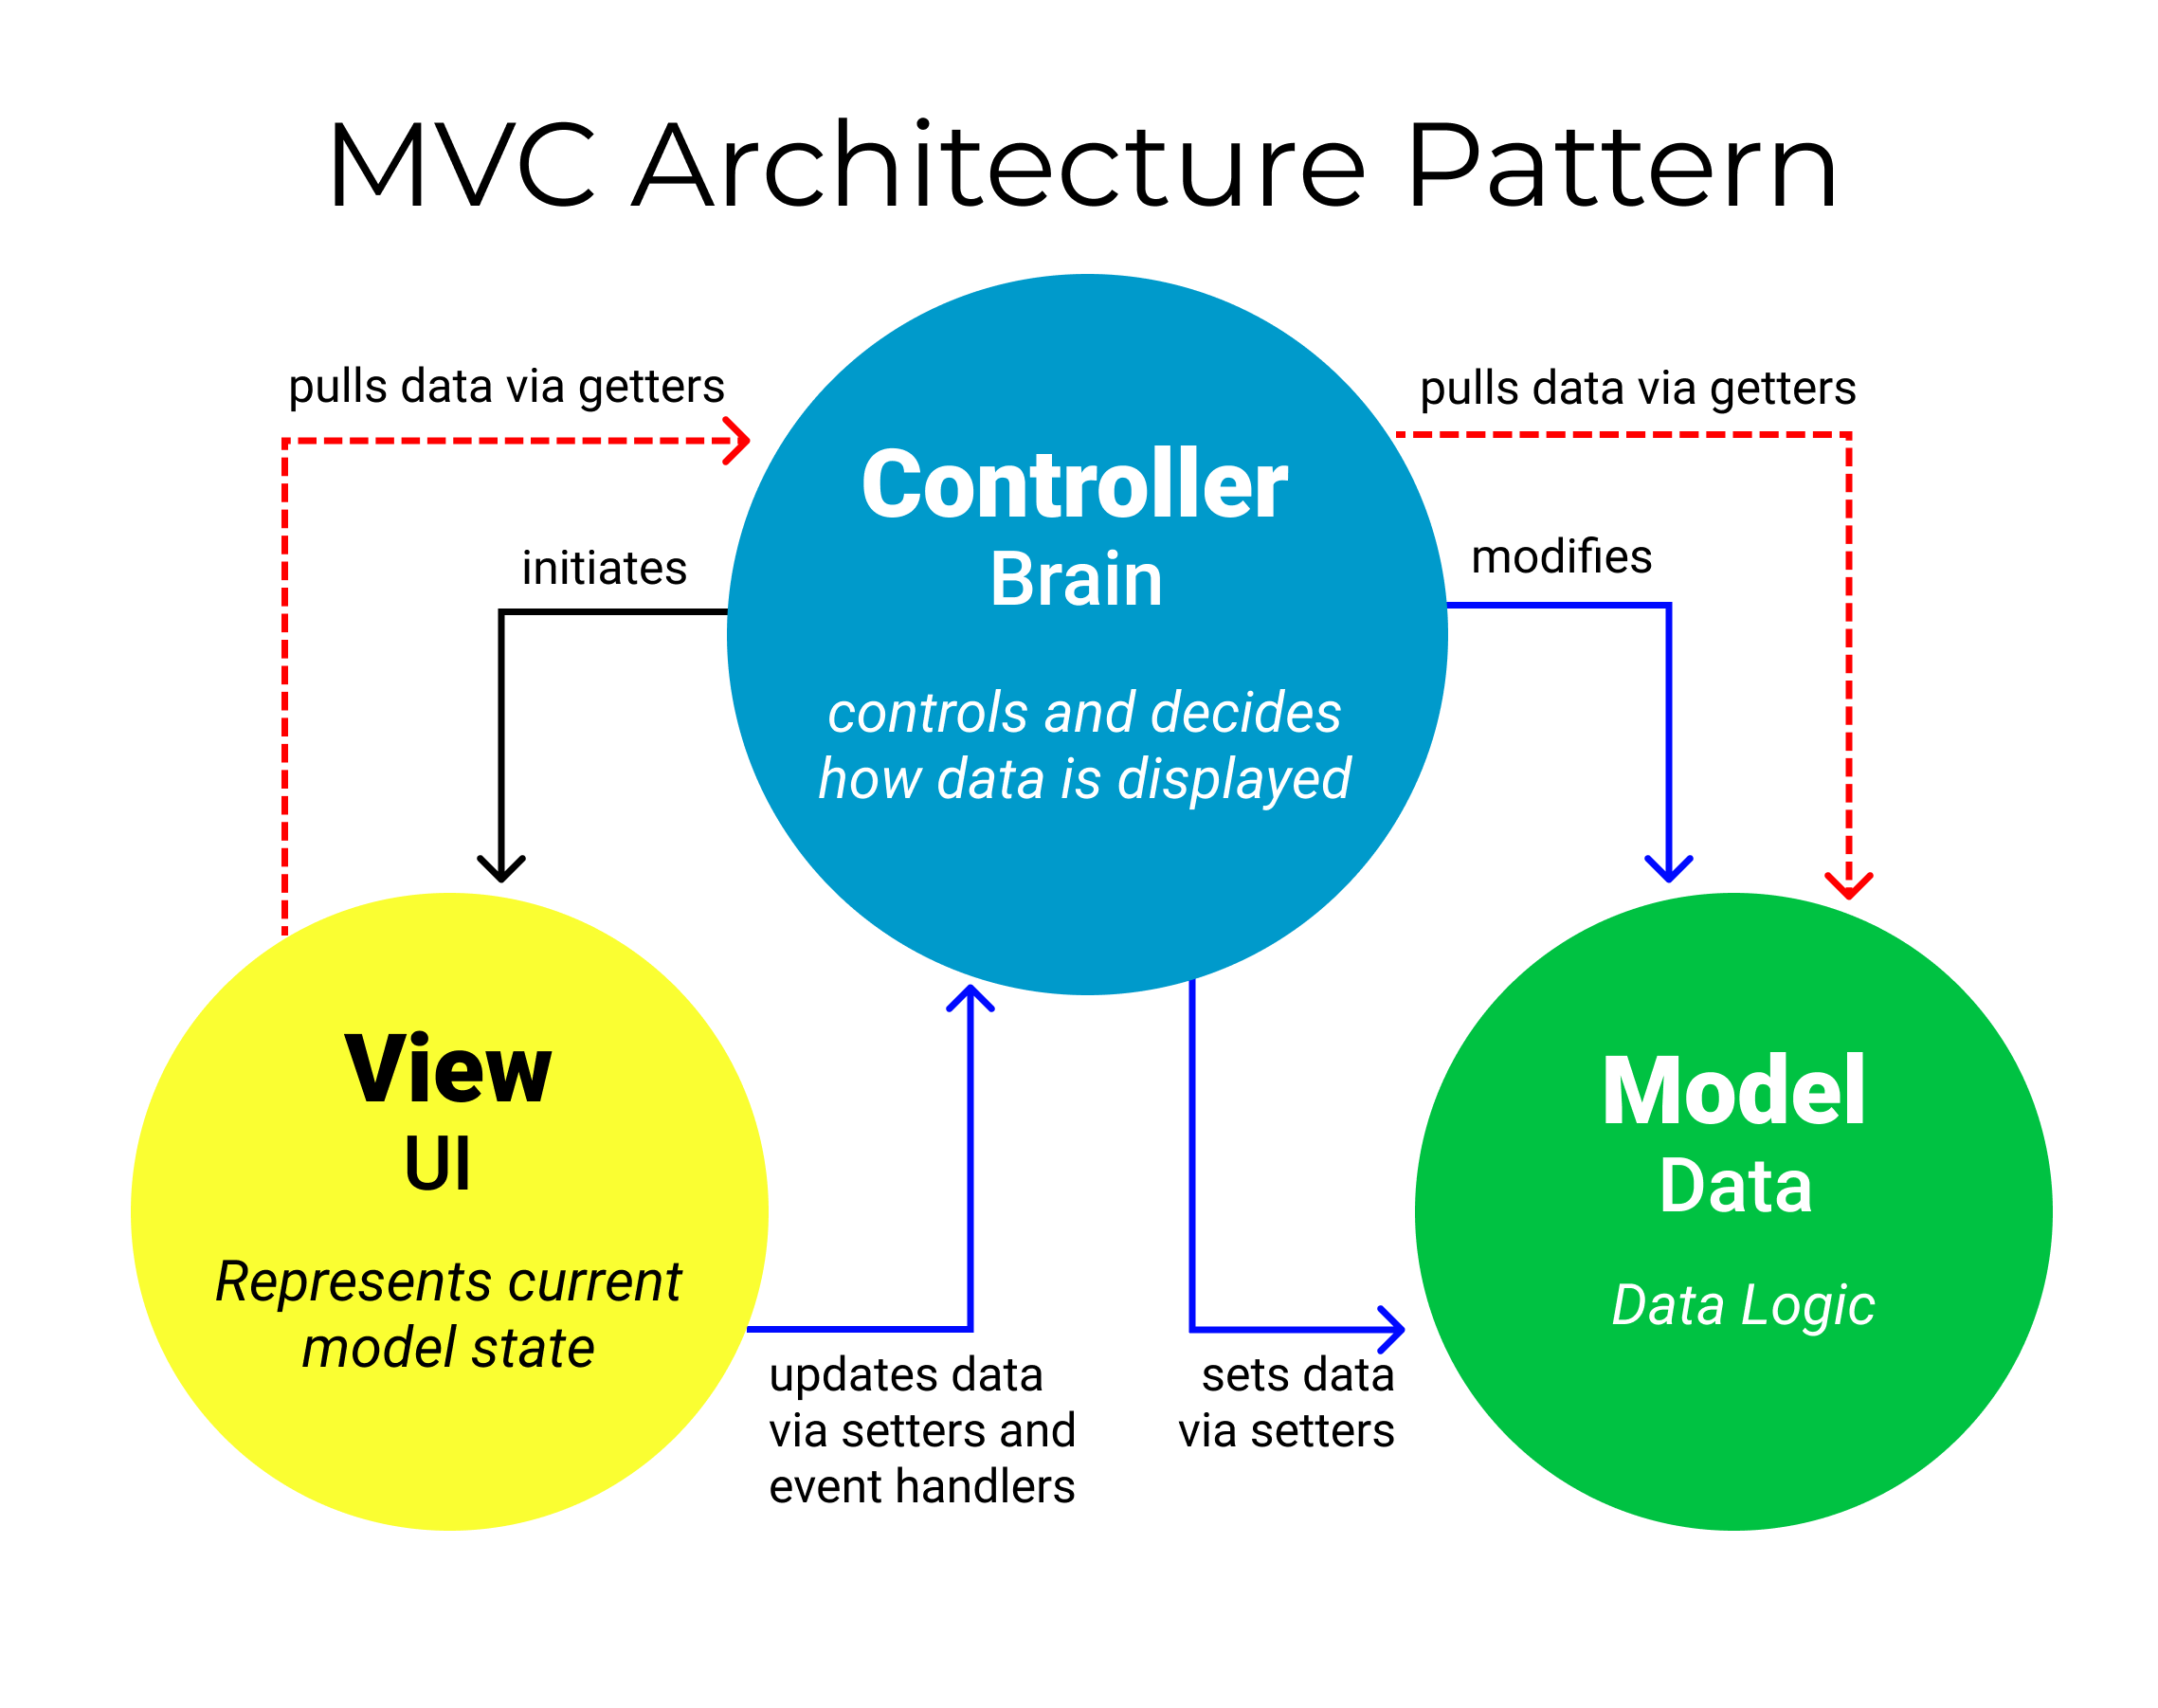
\includegraphics[width=0.90\textwidth]{MVC3.png}
	\end{center}
	\caption{Architecture MVC}
	\label{taquin}
\end{figure}

* Le \textbf{\textit{Modèle}} contient uniquement les données pures de l'application, il ne contient
aucune méthode describant comment afficher les données à l'utilisateur et est plus ou moins 
complétement isolé de la vue.

* La \textbf{\textit{Vue}} présente les donnée du modèle à l'utilisateur. La vue sait comment acceder 
aux données du modèle mais n'en connait ni leur signification ni en quoi l'utilisateur peut en faire.

* Le \textbf{\textit{Contrôleur}} existe entre le modèle et la vue. Il agit sur le modèle en fonction 
des demandes de l'utilisateur.

\subsubsection{Avantages}
L'architecture dispose de plusieurs avantages :
\begin{itemize}
    \item La Séparation des tâches, séparer la logique métier, l'interface utilisateur et la dynamique du système.
    \item Plusieurs développeurs peuvent travailler simultanément sur le Contrôleur, la vue ou modèle.
    \item Permet la création de multiples vues pour un unique modèle.
    \item La Reutilisabilite impliquant ainsi un gain en temps.
\end{itemize}

\subsubsection{Désanvantages}
Néanmoins des désavantages existent :
\begin{itemize}
    \item La navigation de l'architecture devient plus complex car elle introduit un niveau supplémentaire
    d'abstraction.
    \item Un nombre plus grand de fichiers supplémentaires à manipuler.
\end{itemize}

\section{Mise en place de MVC dans le cadre du projet}
\subsection{Arborescence du projet}
L'application est organisée de la manière suivante:
\begin{figure}[h!]
	\begin{center}
		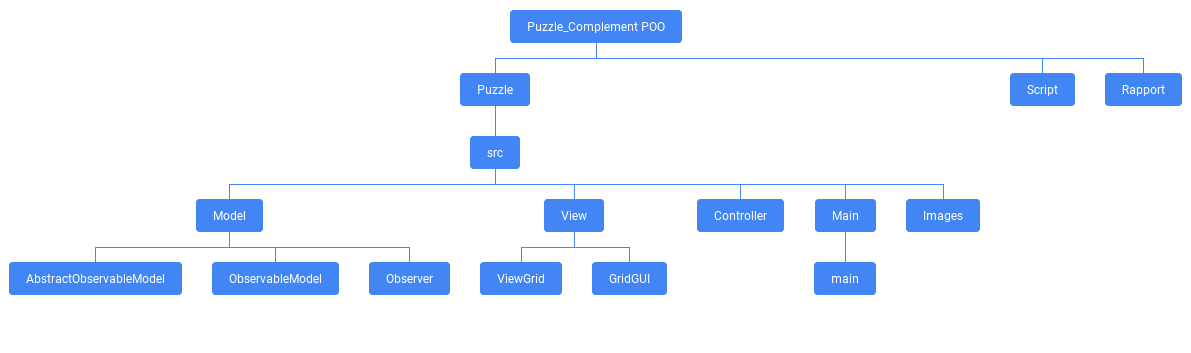
\includegraphics[width=1.2\textwidth]{chart1.png}
	\end{center}
	\caption{Arborescence Projet}
	\label{arbre}
\end{figure}
Comme nous pouvons le voir le projet est composé principalement de trois répertoires:
\begin{itemize}
	\item Script : contenant les différents script
	\item Rapport :  contenant le rapport du projet
	\item src : composé en cinq packages dont \textbf{\textit{model, view, controller}} reprenant ainsi l'architecture MVC.
	Un sous package \textbf{\textit{main}} contenant l'exécutable et repertoire image contenant les différentes images.
\end{itemize}
\newpage
\subsection{Diagramme UML}
Dans le projet il nous a été demandé d'utilisé le design pattern MVC. Il a été implémenté de la manière suivante:
\begin{figure}[ht!]
	\begin{center}
		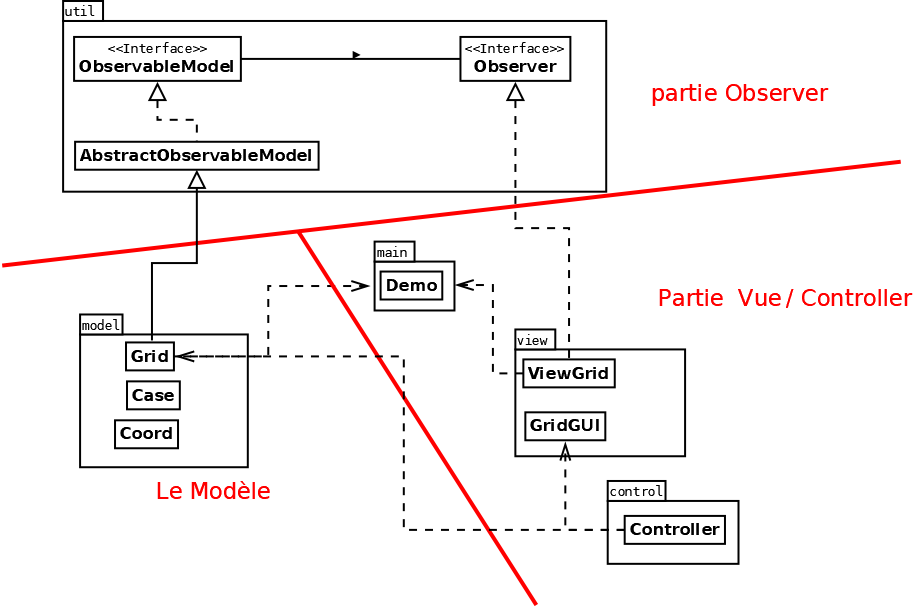
\includegraphics[width=1\textwidth]{puzz.png}
	\end{center}
	\caption{Diagramme de l'application}
	\label{DA}
\end{figure}
\newpage
\subsubsection{Model}
Le modèle est essentiellement la classe Grid ou se place la totalité de la logique. Tous
les traitements restent identiques quelques soit le mode d'affichage souhaité. Les classes Coord et Cases peuvent être considérées comme étant des composantes.
\begin{figure}[h!]
	\begin{center}
		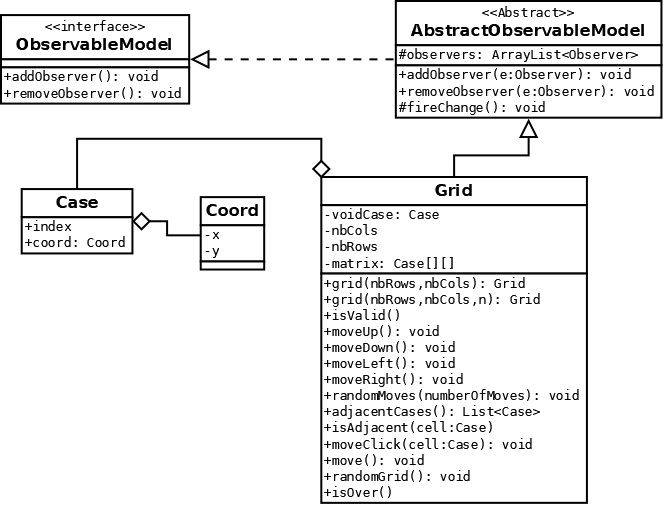
\includegraphics[width=1\textwidth]{model_puzzle.png}
	\end{center}
	\caption{UML du modèle}
	\label{model}
\end{figure}	

Comme nous pouvons le voir la classe Grid hérite de AbstractObservableModel permettant ainsi aux observers d'être notifié à chaque fois que son état change grace à la méthode fireChange().

\newpage
\begin{lstlisting}[tabsize=3,gobble=3]
	protected void fireChange() {
		for(Observer e : observers) {
			e.updateModel(this);
		}
\end{lstlisting}		
\subsubsection{View + Controller}
\begin{figure}[h!]
	\begin{center}
		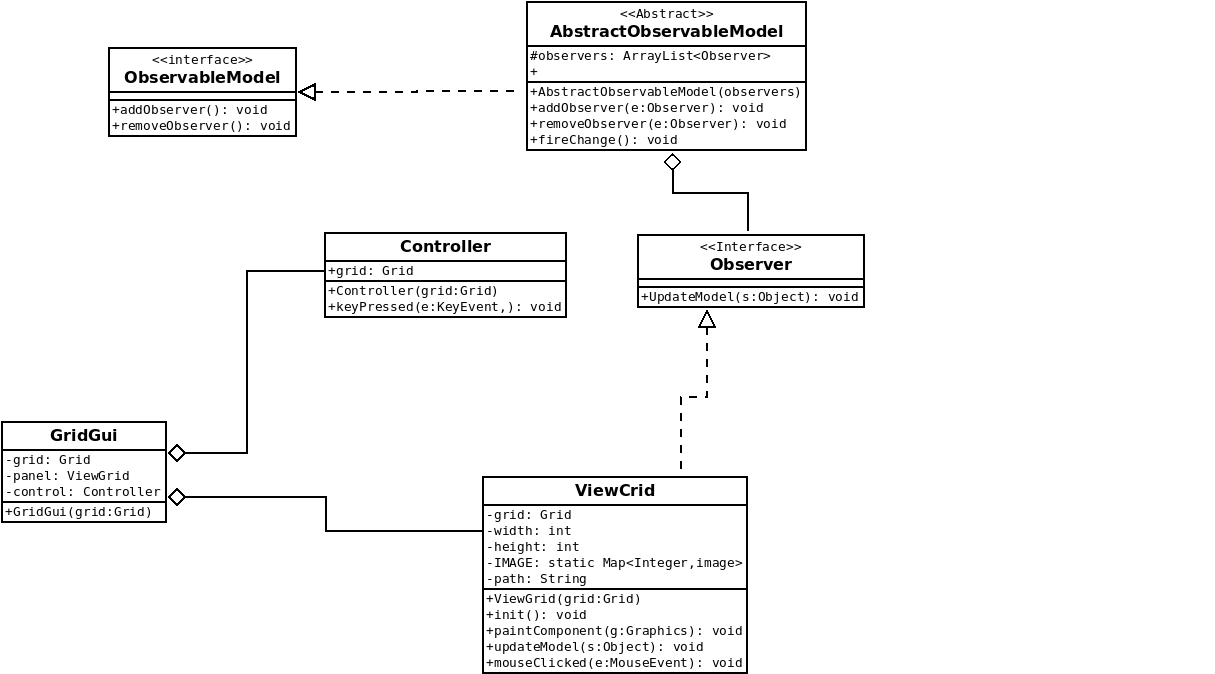
\includegraphics[width=1.3\textwidth]{view.png}
	\end{center}
	\caption{UML View et Controller}
	\label{view}
\end{figure}
La classe \textbf{ViewGrid} s'abonne au modèle en implémentant l'interface \textbf{Observer}
et en prenant bien le modèle \textbf{Grid} comme attribut. Ainsi à chaque changement d'état 
la vue est notifiée et se met à jour.

\textbf{GridGUI} est la frame assurant l'affichage de l'application. 

La classe \textbf{Controller} permet de faire déplacer une case en utilisant les fléches directionnelles.

\section{Eléments techniques}
\subsection{Grid}
Commençons par parler de la classe \textbf{Grid}. En effet il nous a été demandé de faire en sorte que le puzzle soit mélangé mais de sorte qu'il soit quand même solvable.
En effet un méthode brute-force avec une utilisation de chiffres randomment générés aller à coup sur résulter à la creation d'un puzzle dont il est impossible de résoudre. Pour contourner ainsi ce problème rentre en scène la méthode \textbf{\textit{\underline{randomMoves}}}.

Elle prends un certains nombre de moves à faire et génére un chiffre random entre 0 et 4 exclus avec 0 étant la direction \textit{Nord }, 1 \textit{Sud}, 2 \textit{Est} et \textit{Ouest}. La méthode est faite en sorte de garder en mémoire à chaque le direction précédente empêchant ainsi de faire des allers et retours. Exemple : prendre la direction nord puis la direction sud ce qui revient à ne pas bouger(voir algorithme ci-dessous).
\newpage
	\begin{algorithm}[H]
		\caption{randomMoves(int numberOfMoves):void}
		\KwIn{Grid}
		\KwOut{Shuffled grid}
		$past\leftarrow null$
		
		\While{$numberOfMoves > 0$}{
			$r\leftarrow new$ Randow()

			$nbrRandom \leftarrow r.nextInt(4)$
			\\
			$move \leftarrow null$
			\\
			\uIf{$nbrRandom == 0$ \textbf{and} $past <> 1$}{
				$move \leftarrow UP$

				$past \leftarrow 0$

				$numberOfMoves \leftarrow numberOfMoves - 1$
			}\uIf{$nbrRandom == 1$ \textbf{and} $past <> 0$}{
				$move \leftarrow DOWN$

				$past \leftarrow 1$

				$numberOfMoves \leftarrow numberOfMoves - 1$
			}\uIf{$nbrRandom == 2$ \textbf{and} $past <> 3$}{
				$move \leftarrow LEFT$

				$past \leftarrow 2$

				$numberOfMoves \leftarrow numberOfMoves - 1$
			}\uIf{$nbrRandom == 3$ \textbf{and} $past <> 2$}{
				$move \leftarrow RIGHT$

				$past \leftarrow 3$

				$numberOfMoves \leftarrow numberOfMoves - 1$
			}
		}
	\end{algorithm}
\newpage	
\subsection{ViewGrid}
La méthode \textbf{\textit{\underline{init()}}} assure le découpage de l'image en subimages.
Le découpage est fait en sorte que l'image sera découper en \textbf{n * m - 1} sous images avec n étant le nombre de lignes et m le nombre de colonnes, puis ensuite chacune d'entre elle est stockée dans une \textit{HasMap}. La hauteur et la largeur de chaque sous imges est calculée en fonction de celle de l'image d'origine et des dimensions de la grille(Voir code ci dessous.) 
\begin{lstlisting}[tabsize=2,gobble=1]
	public void init() {
		BufferedImage img = null;
		try {
			img = ImageIO.read(new File(path));
			width = img.getWidth(null) / grid.getNbCols();
			height = img.getHeight(null) / grid.getNbRows();
			for (int j = 0; j < grid.getNbRows(); j++) {
				for (int i = 0; i < grid.getNbCols(); i++) {
					int x=img.getWidth()*i / grid.getNbCols();
					int y=img.getHeight()*j / grid.getNbRows();
					IMAGE.put(grid.getMatrix()[j][i].getIndex(), 
					img.getSubimage(x, y, width, height));
				}
			}
		} catch (IOException e) {
			System.out.println("No image found");
		}
	}
\end{lstlisting}
\newpage
\section{Conclusion}
\subsection{Avis Général}
Ce projet fut trés instructif et nous aura mieux permis de cerner et de se familiariser avec le patter \textbf{MVC}. L'intêret de celui-ci apparait clairement car permettant différentes visualisations du model sans avoir à le changer que cela soit en ligne de commande via des Sysout ou en affichage intétgrale via un interface graphique. Elle permet également un sépération du modèle par rapport au reste rendant les classes composant le modéle réutilisables car n'ayant aucun code ayant rapport avec la vue/controller.
\subsection{Eléments à améliorer}
Bien que tout ce qui a été demandé dans le sujet a été remplit, pas mal de choses restent quand même à améliorer mais faute de temps et du nombre de projet à finir en ce fin semestre
tout ce que l'on souhaité n'a pas pu être accomplit.
Par exemple:
\begin{itemize}
	\item Faire en sorte que la frame se resize en fonction de l'image chargée.
	\item Faire en sorte que l'image s'adapte à la taille de la frame lorsqu'on l'aggrandit.
	\item Faire en sorte que la case survolé par la souris si déplacable soit mise en avant.
\end{itemize}
\end{document}
